\documentclass[a4paper,openright,12pt]{article}
\usepackage[utf8]{inputenc}
\usepackage{graphicx} 
\usepackage{subfigure}
\usepackage[mathscr]{eucal}
\usepackage{titling}
\usepackage{float}
\usepackage{amsmath}
\usepackage{afterpage}
\usepackage{vmargin}
\usepackage[spanish]{babel}
\usepackage{eurosym} 
\usepackage{multirow} 
\usepackage{cite}
\usepackage{url}
\usepackage[colorlinks=true,urlcolor=blue, linkcolor = black, citecolor = blue]{hyperref}


\setlength{\parskip}{1ex} 
\setpapersize{A4}	   %  DIN A4
\setmargins{3cm}    % margen izquierdo
{3.5cm}                     % margen superior
{15cm}                       % anchura del texto
{22.5cm}                   % altura del texto
{10pt}                         % altura de los encabezados
{1cm}                         % espacio entre el texto y los encabezados
{0pt}                           % altura del pie de página
{2cm}                         % espacio entre el texto y el pie de página

\begin{document}

\begin{titlepage}

\begin{center}
\vspace*{-1in}
\begin{figure}[htb]
\begin{center}

\includegraphics[width=8cm]{udc.eps}
\end{center}
\end{figure}

PROGRAMACIÓN DE SISTEMAS 24/25 Q1\\

\begin{figure}[htb]
\begin{center}

\includegraphics[width=5cm]{Images/logo.jpg}
\end{center}
\end{figure}

\vspace*{1in}
\begin{Large}
\textbf{Juego de air hockey con pantalla dividida} \\
\end{Large}

\vspace*{2.5in}

\begin{large}
\raggedright
\textbf{Autores:}\\ José Manuel Fernández Montáns (j.m.fmontans@udc.es) \\
Mateo Rivela Santos (mateo.rivela@udc.es)\\
Hugo Mato Cancela (hugo.matoc@udc.es)\\
\textbf{Persona de contacto:} Hugo\\
\textbf{Fecha:}\textit{ A Coruña, 20 de Enero 2025}\\
\textbf{Versión:}\textit{5.0}\\
\textbf{Nombre de la aplicación:} \textit{Space Rend Hockey}\\
\textbf{Github:} \url{https://github.com/Hugoomv/TT_PS_Grupo-Q1.1_24-25}\\
\end{large}

\end{center}
\end{titlepage} 

\newpage

\addtocontents{toc}{\hspace{-7.5mm} \textbf{Capítulos}}
\addtocontents{toc}{\hfill \textbf{Página} \par}
\addtocontents{toc}{\vspace{-2mm} \hspace{-7.5mm} \hrule \par}

\pagenumbering{empty}

\tableofcontents

\vspace{5cm}

\begin{flushright}
\begin{table}[hbtp]
\begin{center}

\caption{Tabla de versiones.}
\label{tabla:versiones}
\small
\vspace{1ex}

\begin{tabular}{|c|c|l|}
\hline
Versión & Fecha & Autor \\
\hline \hline
0.1 & 10/10/24 & Hugo\\ \hline
1.0 & 21/10/24 & Hugo\\ \hline
1.1 & 10/11/24 & Hugo\\ \hline
1.2 & 13/11/24 & Hugo\\ \hline
2.0 & 16/11/24 & Hugo\\ \hline
3.0 &  1/12/24 & Hugo\\ \hline
4.0 & 24/12/24 & Hugo\\ \hline
5.0 & 16/01/25 & Hugo\\ \hline

\end{tabular}

\end{center}
\end{table}
\end{flushright}

\newpage
\pagenumbering{arabic}


%%%%%%%
%%%%%%%
\section{Introducción}\label{cap.introduccion}

%%
\subsection{Objetivos}
El objetivo principal será trabajar con una pantalla dividida con una baja latencia y gestionar los rebotes para una pelota que viaja entre dispositivos y añadir un menú.

Podemos añadir notificaciones para que se una alguien a la partida, añadir un ranking, la pelota que aumente de velocidad con cada rebote de forma indefinida, ver las personas conectadas al juego, poner un estado a cada persona en base a si está en línea o no, o si ya está en una partida.
%%
\subsection{Motivación}
Intención de experimentar con traspaso de datos entre dispositivos e interacción de elementos de la aplicación con la pantalla del dispositivo. 
%%
\subsection{Trabajo relacionado}
Existen aplicaciones similares, como es el caso de juegos de air hockey online. Nuestra aplicación busca conectar dos dispositivos de forma remota, a diferencia de las otras aplicaciones, que apuestan por una pantalla dividida para dos jugadores. Destacar que la base del juego es muy parecida, pero sin tener que conectar pantallas.

%%%%%%%
%%%%%%%
\section{Análisis de requisitos}

%%
\subsection{Funcionalidades}
Conectar dos teléfonos, cada uno mostraría una mitad del campo completo, de forma que los elementos en los que cada usuario se tiene que fijar pueden ser de mayor tamaño.
 
Los mazos con los que cada uno tiene que golpear el disco se controlarían con un solo dedo, apareciendo en la parte de la pantalla donde se mantiene este.
 
El disco, al ser golpeado por uno de los mazos, se mueve en una trayectoria determinada por el ángulo (y, preferiblemente, fuerza) del impacto, pudiendo ser alterada al chocar con los límites del campo, que corresponderían a los bordes del dispositivo.
%%
\subsection{Prioridades}
Lo principal sería lograr la conexión entre dispositivos, pasar los datos de forma correcta y apropiada, que el disco pase y rebote para implementar el juego de air hockey.
Primero, se implementará el traspaso de objetos entre pantallas y dispositivos con conexión mediante wifi-internet usando Firebase.
Luego, trabajaremos con rebotes y bordes de la pantalla como paredes.
Una vez realizado lo más básico, añadiremos una pantalla de menú y ajustes. 

%%%%%%%
%%%%%%%
\section{Planificación inicial}

%%
\subsection{Iteraciones}
Aquí se definen los prototipos de nuestro proyecto y las funcionalidades principales que trabajamos en cada prototipo. Se implementarán en el orden establecido:
\begin{description}
\item[P1:] Pasar un objeto entre dos dispositivos conectados por Wifi-internet usando Firebase.
\item[P2:] Implementar los rebotes y los bordes de la pantalla del dispositivo como paredes en un modo para un jugador.
\item[P3:] Añadimos una maza que el usuario puede manejar y que rebota con la pelota. Sigue siendo en modo para un jugador.
\item[P4:] Añadir un menú con el que acceder a la pantalla de ajustes. Unión de funcionalidades de P1 y P2: un disco que rebota y se transporta entre dos pantallas al atravesar el borde superior. 
\end{description}
%%
\subsection{Responsabilidades}
\begin{description}

\item[Físicas:] Mateo 
\item[Conexión y Visualización:] José Manuel
\item[Visualización y Entregable:] Hugo
\end{description}

%%
\subsection{Hitos}
\begin{itemize}
\item Crear usuarios en la BD.
\item Login y logout de usuarios.
\item Enviar datos entre dos dispositivos usando Firebase.
\item Establecer una conexión de baja latencia entre ambos dispositivos.
\item Implementar rebotes.
\item Hacer que los bordes de la pantalla funcionen como paredes.
\item Crear un menú con varios ajustes.
\item Crear una partida añadiendo a un jugador mediante invitación.
\item Mostrar un ranking con el número de victorias o puntos.
\end{itemize}

Entregables:
Cada prototipo será una entrega.

%%
\subsection{Incidencias}
No tenemos conocimientos sobre gráficos o físicas por lo que tendremos que aprender y probar todo lo relacionado a eso. Para establecer la conexión se hará uso de Firebase, concretamente RealTimeDatabase \cite{misc-firebase}. En lo relacionado a Android, tomaremos como referencia lo enseñado en clase y la documentación oficial\cite{misc-android-developers}. Por último, en lo relacionado a los gráficos y apartado más visual, Canva \cite{misc-canva}.
\par
En la primera iteración, probaremos la conexión entre dispositivos y que el objeto pasa correctamente entre ellos.
En la segunda, en un prototipo distinto, el objeto debe rebotar contra los bordes de la pantalla de un dispositivo para que funcionen como paredes.
En la tercera, implementamos la maza, que debe responder correctamente al input del usuario, y nos aseguramos de que la pelota rebote correctamente contra esta.
En la cuarta, uniremos las funcionalidades de las dos primeras iteraciones y nos aseguraremos de que funcionan correctamente ambas al mismo tiempo. Finalmente, comprobaremos que, tras haber implementado todo, funciona correctamente.
\par
En caso de que alguien enferme repartiremos el trabajo asignado a esa persona entre los demás integrantes del grupo.

%%%%%%%
%%%%%%%
\section{Diseño}
\subsection{Arquitectura}
Se hará uso de una arquitectura centralizada cliente-servidor. La distribución de trabajo se hará entre el servidor (Firebase) y el cliente (el usuario de nuestra app). El servidor almacena la información de los usuarios y los mensajes que envían. Guardará datos como si el usuario está conectado o no, su id (único para cada uno), nombre, correo y contraseña. El cliente revisa el usuario actual, con el que estamos logueados, en el servidor y tiene un listener que escucha los cambios, como son los mensajes recibidos por otros usuarios.

\subsection{Persistencia}
Respecto a qué información almacenaremos, los jugadores obtendrán la posición de la pelota una vez sale de la pantalla de su oponente. Además, cada uno guardará dónde está situada su propia maza en caso de que esté siendo usada. El servidor guardará las coordenadas de la pelota. \\
Mientras el usuario está conectado, podrá recibir datos, invitaciones o mensajes y se mostrará como online. Una vez que esté fuera de línea, no será posible que reciba nada de lo anterior. Cuando vuelva a conectarse, se actualizará y cargará los mensajes que recibió mientras estaba offline.

\subsection{Vista}
En lo que respecta al diseño de la aplicación, tendremos una actividad principal desde la que se llaman a los demás componentes al cumplir ciertas condiciones:\\

\begin{itemize}
    \item Se llama a LoginActivity en caso de que no haya un usuario con sesión abierta en la app. Tiene los siguientes elementos:
    \begin{itemize}
        \item TextView con un mensaje que indica la necesidad de iniciar sesión para usar la aplicación.
	\item Imagen con el icono de la app.
        \item Botón de inicio de sesión, que abre un AlertDialog con los campos para introducir los datos del usuario y un botón para registrar un nuevo usuario
        \item Botón de registro, que abre un AlertDialog similar al abierto por el botón de inicio de sesión
    \end{itemize}
    Tras iniciar sesión, se devuelve al usuario a la actividad principal que cuenta con dos botones y un TextView:
    \begin{itemize}
       \item El TextView muestra una lista con los datos de los 10 jugadores con mayor número de victorias. 
        
        \item El botón de Top Players oculta o revela el TextView, además de actualizar la información del mismo.
        
        \item El botón de mandar invitación abre un AlertDialog con un ListView con los usuarios activos, al seleccionar uno y hacer click en el botón OK, manda una invitación al usuario en forma de AlertDialog.
    \end{itemize}

    \item Se llama a GameActivity al comenzar una partida. Esta actividad gestiona el manejo del juego mediante un view personalizado, que muestra todos los elementos y actualiza sus respectivas posiciones cada cierto tiempo.

    \item Se mostrarán ajustes al presionar el botón correspondiente en el menú. Mostrará un menú con varias opciones para modificar la configuración de la aplicación mediante SharedPreferences, cerrar sesión o borrar el usuario. Las dos últimas opciones muestran un AlertDialog para confirmación, y el de borrado de usuario requiere además la contraseña del mismo.

\end{itemize}


\subsection{Comunicaciones}
La comunicación en este juego es una parte fundamental. Para ello, buscamos un sistema de baja latencia. Para esta conexión, se contará con un servidor central al que cada cliente se conectará por internet (Firebase, concretamente RealTimeDatabase); de esta forma, se gana en rango de uso (rango global). Este servidor será usado para el envío de datos en la partida y para las invitaciones entre usuarios. Existe un claro problema y es que el servidor del que se va a hacer uso es gratuito y, por lo tanto, la latencia va a ser bastante alta. Sin embargo, hemos llegado a la conclusión de que no es crítico para este proyecto porque, como cada usuario en una partida solo va a ver su pantalla a priori. En el caso de que ambos jugadores estén juntos físicamente, la latencia sería notable.

\subsection{Sensores}
Se hace uso de la pantalla táctil, con este se implementará el movimiento del mazo en cuestión. Es un dispositivo que detecta y responde al contacto físico o la presión sobre su superficie, en este caso no se hará uso de la detección de la presión. Para la implementación del rebote se puede tener o no en cuenta la velocidad con la que se desplaza en contacto con el panel táctil, pero no es algo que vayamos a implementar en nuestro caso desde a priori.

\subsection{Trabajo en background}
Se han establecido listeners para detectar cambios en los datos pertinentes de la base de datos en tiempo real, por lo que se actualizarán únicamente cuando sea necesario. Se usa Firebase para trabajar con una comunicación y latencia en tiempo real. Los datos de la posición y ángulo de la pelota se envían una vez sale de la pantalla del usuario y pasa al otro jugador. Esta política de funcionamiento nos permite trabajar usando menos datos, haciendo el proceso más sencillo y rápido. Adicionalmente, en el GameActivity se usan hilos para ejecutar el juego.

\section{Arquitectura Propuesta}
La aplicación comenzó siendo monolítica y cambiará a CLEAN Arquitecture. En la primera iteración hay una actividad principal que incluye todo, user y UsersAdapter para el ListView que muestra los usuarios conectados. Según avanzan las iteraciones, se modifica la organización del código, haciendo uso de varias clases e interfaces, para organizar. Esto se consigue separando las funciones relacionadas a Firebase a nuevos arhcivos y clases. Para la creación de las interfaces y gestionar el menú se hará el mismo procedimiento.

\section{Diseño e implementación}
\subsection{1ª iteración}
Se ha creado una aplicación con una MainActivity, UsersAdapters y User. Partimos de un diseño monolítico, que en un futuro pasará a ser CLEAN Arquitecture. En la MainActivity está la mayor parte del código, como es la UI. La interfaz incluye en la parte superior un TextView que mostrará los mensajes que recibamos de otros jugadores. Después, un EditText donde escribir el mensaje que queremos enviar a otros jugadores. Más abajo, están cuatro botones. Por último, un TextView con nuestro nombre de usuario y el email. Este último TextView no mostrará nada si el usuario no está logueado. Además, se ha añadido un toast para informar al usuario si hay problemas al iniciar sesión, conectarse...
A continuación se explica el funcionamiento de los botones:
\begin{itemize}
    \item Send: muestra un desplegable con los usuarios conectados a los que podemos enviar un mensaje. Deshabilitado si el usuario no ha iniciado sesión.
    \item Logout: permite cerrar sesión.
    \item Login: iniciar sesión. Muestra AlertDialog para introducir los datos, correo y contraseña. Además, aparece un botón para cambiar a register. Deshabilitado si el usuario ya ha iniciado sesión.
    \item Register: registrar usuario. Muestra un AlertDialog similar al de login y también tiene el botón para alternar a login. Deshabilitado si el usuario ya ha iniciado sesión.
\end{itemize}
En la figura 1 se muestran unas imágenes de la interfaz. 
\begin{figure}[htp]
    \centering
    \begin{minipage}{0.3\textwidth}
        \centering
        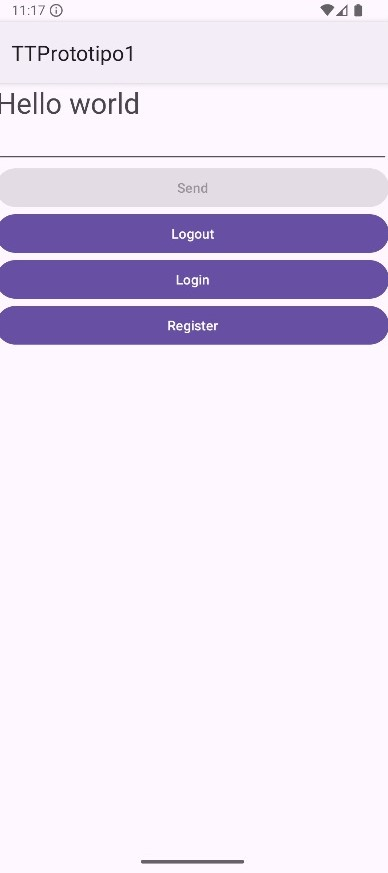
\includegraphics[width=0.6\textwidth]{Images/Vista_It1.jpg} 
        \caption{Pantalla de inicio}
        \label{fig:Pantalla de inicio}
    \end{minipage}
    \hfill
    \begin{minipage}{0.3\textwidth}
        \centering
        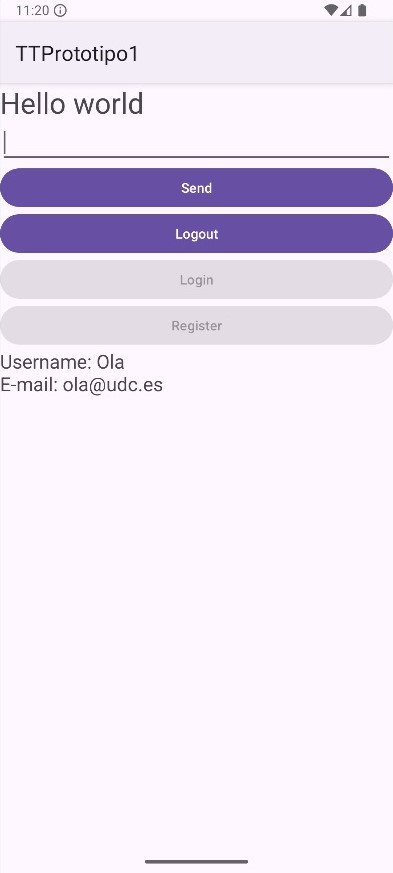
\includegraphics[width=0.6\textwidth]{Images/Vista_It1_2.jpg} 
        \caption{Pantalla una vez iniciada sesión}
        \label{fig:Pantalla una vez iniciada sesión}
    \end{minipage}
    \caption{Pantallas de la primera iteración}
    \label{fig:primera iteración}
\end{figure}

UsersAdapters y Users es usado para la implementación del ListView que muestra los usuarios conectados (tras pulsar Send). La app se conecta a Firebase, donde se han creado varios usuarios para comprobar que funciona correctamente, con su login y logout, y se ha implementado el envío de mensajes, lo que representaría a los primeros hitos.
Finalmente, también se ha inicializado la base de datos haciendo uso del json.

\subsection{2ª iteración}
Para esta iteración, la intención era crear un nuevo prototipo donde ver el funcionamiento de las físicas de la pelota, como se comenta en el apartado de iteraciones. Los rebotes de la pelota son una mecánica fundamental del juego, por lo que se debe lograr lo antes posible. Se ha decidido unir ambos prototipos, debido a que se considera que crear uno separado solamente para el apartado de físicas era poco productivo, incómodo e innecesario. \\ 
Al mismo tiempo que se implementaban las físicas, otra parte del equipo que estaba libre, decidió actualizar la interfaz de usuario para mejorar su aspecto. Para ello se ha hecho uso de estilos, buscando homogeneidad y separación de los bordes y otros elementos. También se ha añadido un menú lateral donde ver la foto de perfil (por implementar), la configuración (de momento vacía) y poder salir de la aplicación. En un futuro, puede que se modifique por un cambio de diseño y por la comodidad del usuario. Además, la interfaz principal ahora es un Drawer donde está el layout anterior y la toolbar con el botón para el menú lateral.\\ 
Por último, también se comenzó con la transición para cambiar el diseño monolítico de la aplicación. Las funciones responsables de la creación del menú están en un fichero distinto llamado UIHelper. Estas incluyen la creación del menú lateral, el botón del menú en el toolbar, la gestión del drawer y las opciones del menú.
La figura 2 contiene 2 capturas donde se ve el nuevo diseño de la UI y el menú lateral.

\begin{figure}[htp]
    \centering
    \begin{minipage}{0.3\textwidth}
        \centering
        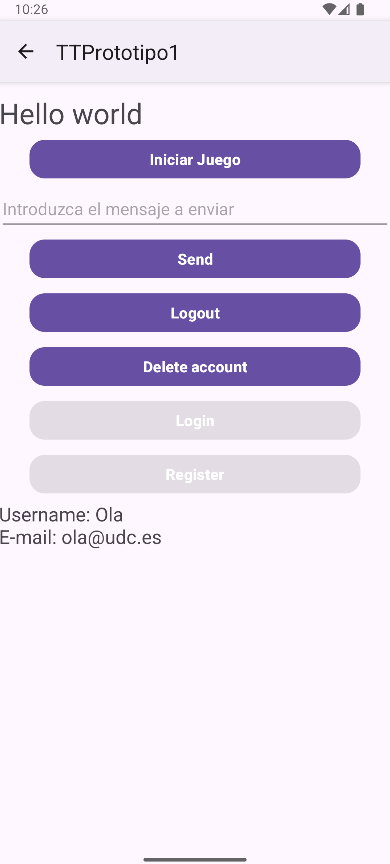
\includegraphics[width=0.6\textwidth]{Images/Vista_It2.png} 
        \caption{Pantalla de inicio}
        \label{fig:Pantalla de inicio}
    \end{minipage}
    \hfill
    \begin{minipage}{0.3\textwidth}
        \centering
        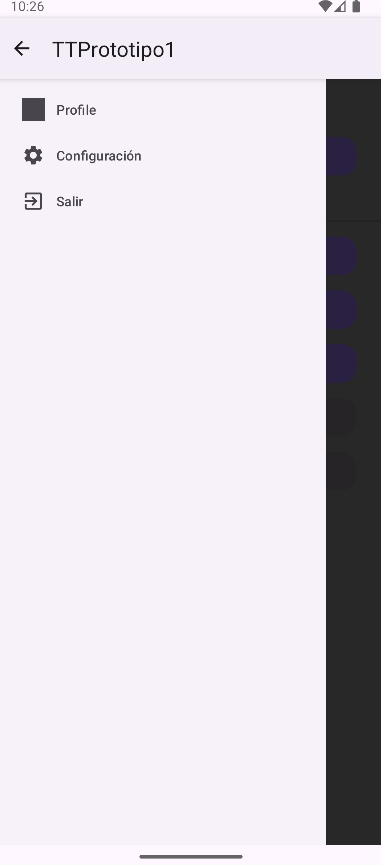
\includegraphics[width=0.6\textwidth]{Images/Vista_It2_2.png} 
        \caption{Menú lateral}
        \label{fig:Menú lateral}
    \end{minipage}
    \hfill
    \begin{minipage}{0.3\textwidth}
        \centering
        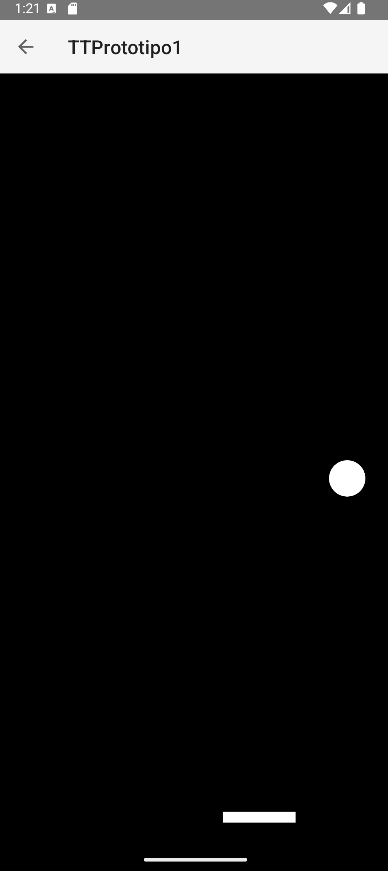
\includegraphics[width=0.6\textwidth]{Images/Vista_It2_3.png} 
        \caption{Pantalla de juego}
        \label{fig:Pantalla de juego}
    \end{minipage}
    \caption{Pantallas de la segunda iteración}
    \label{fig:segunda iteración}
\end{figure}

\subsection{3ª iteración}

De cara a cumplir con lo planeado para el {$3^{er}$} entregable, se ha actualizado el juego para que incluya la maza (como se especificó en los hitos), que permite al usuario interactuar con la pelota de forma mucho más similar al juego final. Además, se ha iniciado el trabajo en el apartado de enviar el disco entre dos pantallas. Ahora, cuando toca la parte superior de la pantalla, la aplicación supone que ya se ha salido de nuestro campo. La lógica que envía los datos por Firebase y se encarga de recibir los datos en el otro jugador aún está por implementar.\\
En la interfaz, se han actualizado los colores principales de la app, junto a pequeños retoques en la toolbar. También se modificó el menú lateral, que ahora es de tipo ModalNavigationDrawer. Este es el más común y resultará familiar al usuario. Se abre desde la izquierda y no ocupa toda la pantalla. Se ha añadido un imageView, que en un futuro servirá para las imágenes de perfil de los usuarios. Adicionalmente, están varias opciones básicas (sin implementación) y la opción de salir de la app. Por último, como se pueden ver en las imágenes de la figura 7, se ha cambiado la SplashScreen (pantalla de carga inicial, al abrir el juego) con una animación (animated vector) sobre un icono de prueba y un nuevo tema que se aplica a la aplicación en el manifiesto.

\begin{figure}[htp]
    \centering
    \begin{minipage}{0.3\textwidth}
        \centering
        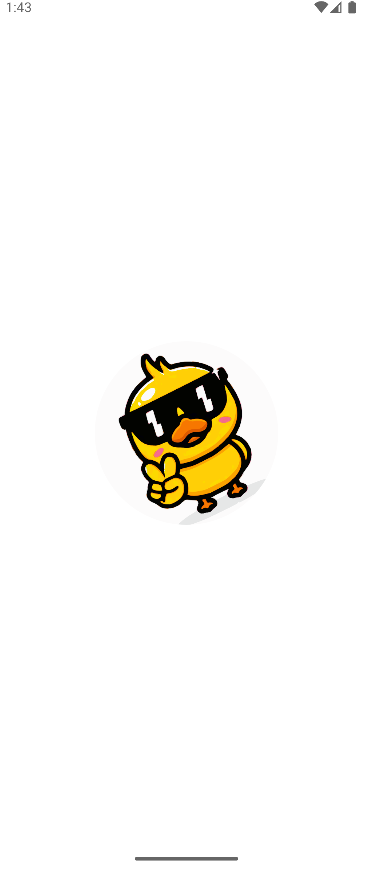
\includegraphics[width=0.6\textwidth]{Images/Vista_It3_3.png} 
        \caption{Nueva SplashScreen}
        \label{fig:Nueva SplashScreen}
    \end{minipage}
    \hfill
    \begin{minipage}{0.3\textwidth}
        \centering
        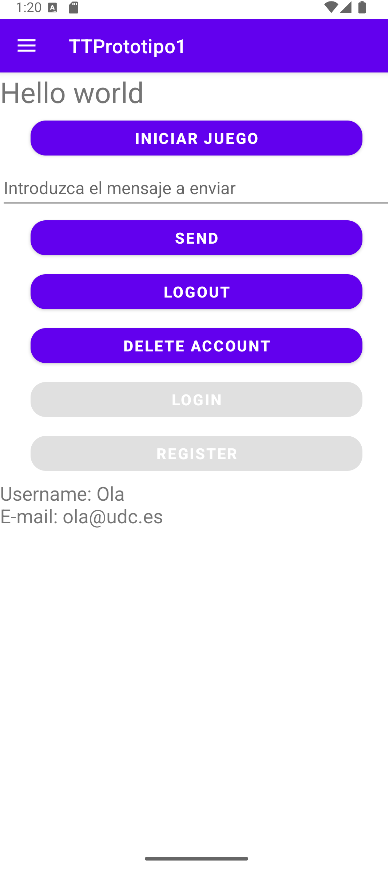
\includegraphics[width=0.6\textwidth]{Images/Vista_It3.png} 
        \caption{Pantalla de inicio}
        \label{fig:Pantalla de inicio}
    \end{minipage}
    \hfill
    \begin{minipage}{0.3\textwidth}
        \centering
        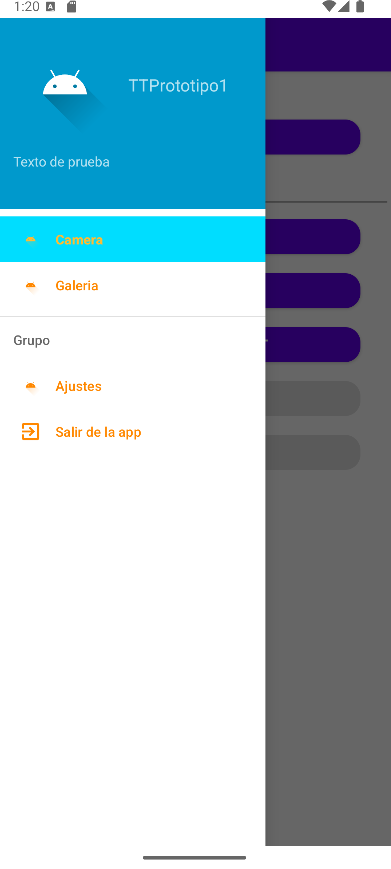
\includegraphics[width=0.6\textwidth]{Images/Vista_It3_2.png} 
        \caption{Nuevo menú lateral}
        \label{fig:menú lateral}
    \end{minipage}
    \caption{Pantallas de la tercera iteración}
    \label{fig:tercera iteración}
\end{figure}

\subsection{4ª iteración}
En este punto la app está casi completa. Como se puede ver en las capturas, en el apartado gráfico, se han actualizado los íconos de la app en Resources, la SplashScreen ahora usa el ícono de la app, el menú ahora tiene nuevos botones para cerrar sesión, ajustes, borrar cuenta, salir de la app y un icono en la cabecera personalizable; se ha añadido modo oscuro, soporte para el inglés. Además, la nueva pantalla de inicio incluye el icono de la app, los botones adoptan el diseño correspondiente, el alert dialog para loguearse o registrarse ha sido actualizado y también hay un ranking de mejores jugadores. \\
De cara a lo relacionado con el juego en sí, ahora para iniciar partida se envía una invitación al otro jugador que puede aceptar o rechazar, se ha añadido un sistema para decidir al ganar en base a puntos y un botón de no molestar que no permite recibir invitaciones y la pantalla de inicio ahora exige estar logueado o crear una cuenta para acceder a la app.

\begin{figure}[htp]
    \centering
    \begin{minipage}{0.3\textwidth}
        \centering
        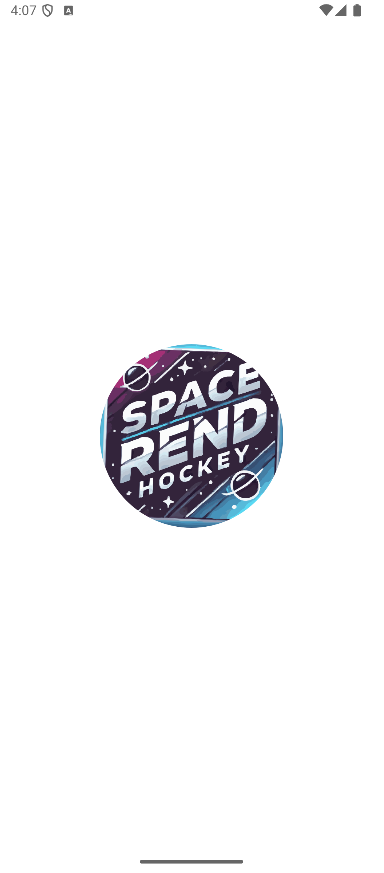
\includegraphics[width=0.6\textwidth]{Images/Vista_It4.png} 
        \caption{SplashScreen actualizada}
        \label{fig:SplashScreen actualizada}
    \end{minipage}
    \hfill
    \begin{minipage}{0.3\textwidth}
        \centering
        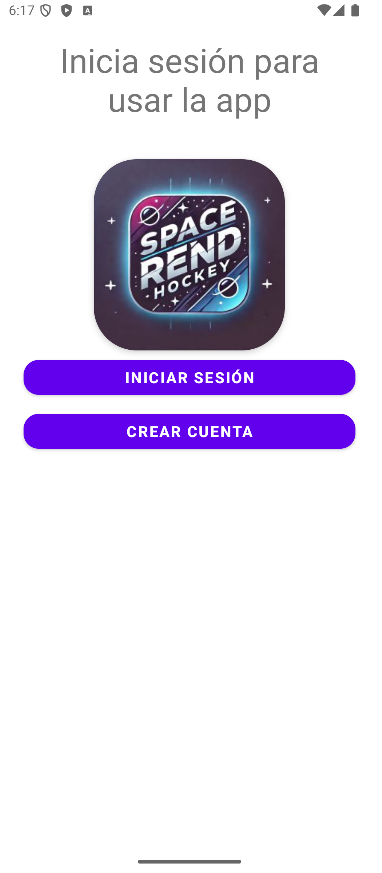
\includegraphics[width=0.6\textwidth]{Images/Vista_It4_1.png} 
        \caption{Nueva pantalla de inicio}
        \label{fig:Pantalla de inicio}
    \end{minipage}
    \hfill
    \begin{minipage}{0.3\textwidth}
        \centering
        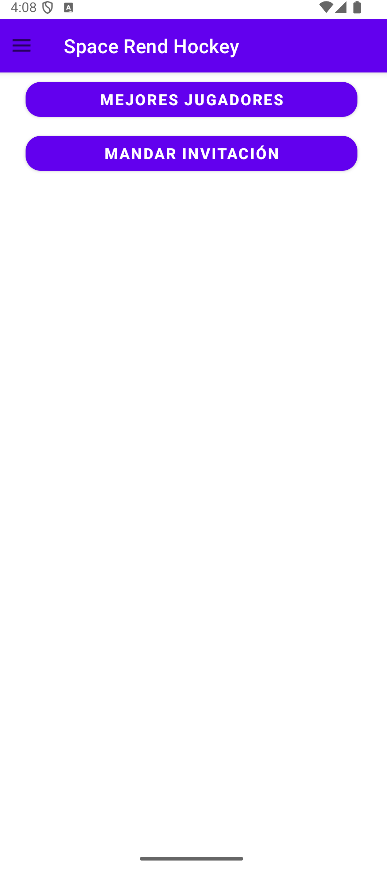
\includegraphics[width=0.6\textwidth]{Images/Vista_It4_2.png} 
        \caption{Pantalla principal}
        \label{fig:pantalla principal}
    \end{minipage}
\end{figure}

\begin{figure}[htp]
    \begin{minipage}{0.3\textwidth}
        \centering
        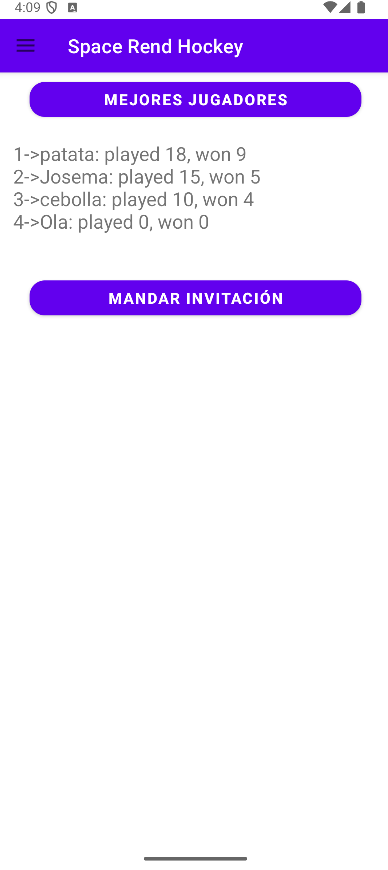
\includegraphics[width=0.6\textwidth]{Images/Vista_It4_3.png} 
        \caption{Nueva leaderboard}
        \label{fig:leaderboard}
    \end{minipage}
    \hfill
    \begin{minipage}{0.3\textwidth}
        \centering
        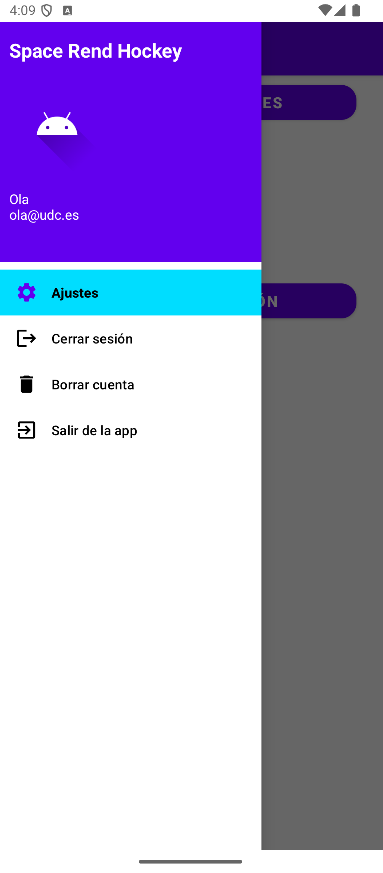
\includegraphics[width=0.6\textwidth]{Images/Vista_It4_4.png} 
        \caption{Menú lateral actualizado}
        \label{fig:menú lateral actualizado}
    \end{minipage}
    \hfill
    \begin{minipage}{0.3\textwidth}
        \centering
        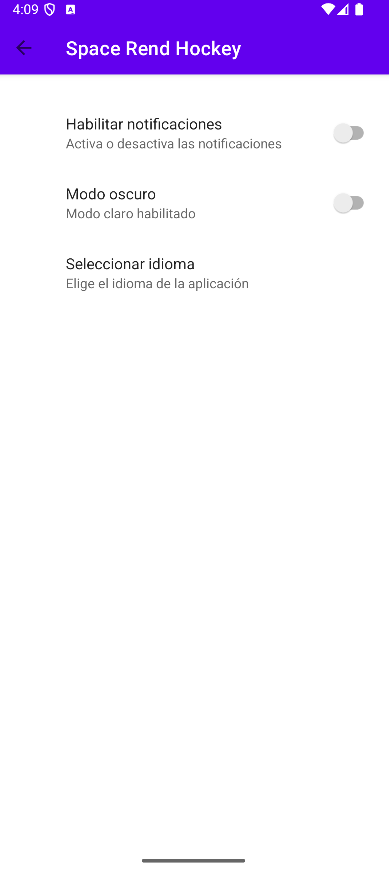
\includegraphics[width=0.6\textwidth]{Images/Vista_It4_5.png} 
        \caption{Ajustes actualizados}
        \label{fig:ajustes actualizado}
    \end{minipage}
\end{figure}


\begin{figure}[htp]
    \centering
    \begin{minipage}{0.3\textwidth}
        \centering
        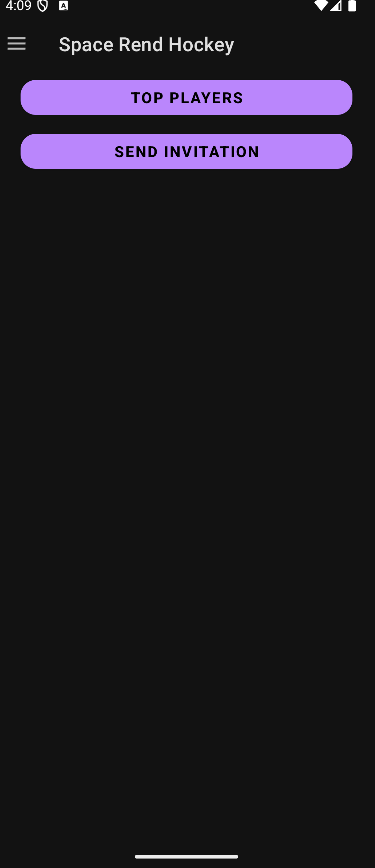
\includegraphics[width=0.6\textwidth]{Images/Vista_It4_6.png} 
        \caption{Inicio}
        \label{fig:pantalla principal}
    \end{minipage}
    \hfill
    \begin{minipage}{0.3\textwidth}
        \centering
        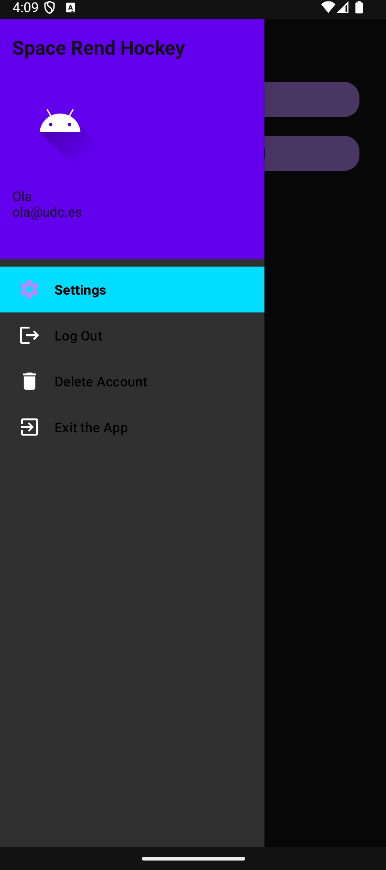
\includegraphics[width=0.6\textwidth]{Images/Vista_It4_7.png} 
        \caption{Menú lateral}
        \label{fig:menñu lateral}
    \end{minipage}
    \hfill
    \begin{minipage}{0.3\textwidth}
        \centering
        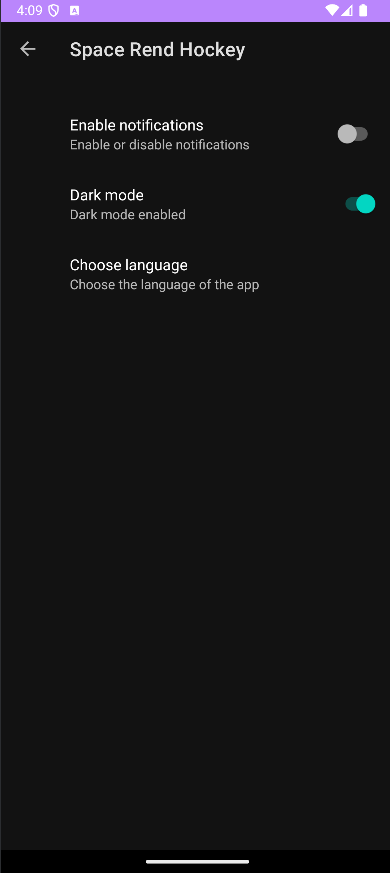
\includegraphics[width=0.6\textwidth]{Images/Vista_It4_8.png} 
        \caption{Ajustes}
        \label{fig:ajustes}
    \end{minipage}
    \caption{Capturas de pantalla de la cuarta iteración}
\end{figure}

\section{Pruebas}
\subsection{$1^{as} \text{ pruebas}$}
Se han usado dos emuladores en la misma máquina para comprobar el funcionamiento de la aplicación. Se ha comprobado el registro de usuarios, el login, el logout, la creación de datos en la base de datos en tiempo real y el paso de mensajes usando Firebase. Adicionalmente, se han usado varios equipos distintos y se han comunicado varias apps de emuladores y equipos diferentes.

\subsection{$2^{as} \text{ pruebas}$}
Para el segundo hito se han realizado comprobaciones de que la pelota rebota correctamente. Al iniciar el juego, esta se mueve hasta que se cierra esta pantalla. Además, se revisa el estado de la UI tras los cambios, ejecutando todas las funciones comprometidas y verificando su correcto desenvolvimiento. Esto se aplica para el menú lateral, la toolbar y los botones a los que se aplicó un cambio de estilo y/o funcionamiento.


\subsection{$3^{as} \text{ pruebas}$}
Las pruebas para el {$3^{er}$} entregable son básicas. Para la SplashScreen simplemente se revisa que funciona al iniciar app y que se aplica el tema correspondiente después. Para el nuevo menú, se han añadido toast para comprobar que funciona correctamente a pesar de no tener implementación. Finalmente, el juego se testea haciendo uso de la maza y lanzando la pelota a la parte superior de la pantalla.

\subsection{$4^{as} \text{ pruebas}$}
Para esta iteración, se ha revisado el correcto funcionamiento de toda la app. Esto incluye comprobar que se crean, actualizan y borran los usuarios de forma correcta en la BD, para ello, se accede al proyecto en Firebase; la bola se envía correctamente entre dispositivos y el modo no molestar funciona, ejecutando dos emuladores de forma simultánea, y se han probado cambios en la interfaz al pasar a tema oscuro o al inglés. Para ello se ha hecho uso de los botones en la app o ejecutado órdenes de forma directa. También se ha probado que el menú y los botones realizan las acciones asignadas de forma correcta, la tabla de top jugadores muestra los resultados adecuados, se puede cambiar el icono del menú y se guardan las preferencias de forma exitosa. Adicionalmente, para corroborar que los datos son correctos, se han añadido logs o toast en lugares puntuales, principalmente errores.
%%%%%%%

\section{Trabajo futuro}
La app,  si bien es completamente funcional, todavía tiene espacio para mejora. Entre las posibles modificaciones que se podrían realizar en un futuro están las siguientes:

\begin{itemize}

\item Modificar el sistema de invitaciones para que notifique al usuario con notificaciones, de forma que no tenga que tener abierta la aplicación.

\item Modificar la interfaz gráfica: Añadir más animaciones y elementos visuales relacionados con la temática de la aplicación.

\item Proporcionar elementos que aporten feedback auditivo al usuario: Música de fondo (distinta en la actividad principal y los menús y las partidas en sí) o efectos de sonido que resalten sucesos importantes (como rebotes de la pelota).

\item Asignar la foto al usuario y no a la configuración de la aplicación (Storage de Firebase es de pago).

\item Incluir un modo de juego para una persona, que no requiera de conexión a internet o usuarios activos.

\item Publicar la app en la PlayStore.

\end{itemize}

\section{Incidencias destacables en la realización del TT}
Uno de los mayores problemas fue la falta de conocimiento a la hora de afrontar todo lo relacionado con Firebase. Si bien no es muy complejo, este proyecto fue el primer contacto del equipo. Esto supuso varios problemas a lo largo del desarrollo y aumentó el tiempo dedicado a esta parte. Algo similar ocurrió en la creación y manipulación de iconos y animaciones. \\
Además, la gestión y estimación de tareas no fue la óptima. Esto derivó en una mala planificación del tiempo y lo que al principio suponía un proyecto sencillo acabó siendo de mucha mayor envergadura.


\section{Bibliografía}
\bibliographystyle{pfc-fic}
\bibliography{biblio}


\end{document}